
\chapter{Illumination Model}

当光照射到物体表面时,物体会对光发生反射、透射、吸收、衍射、折射、干涉等。其中被物体吸收的部分转化为热。
反射、透射的光会进入人的视觉系统,使我们看见物体。为了模拟仿真这一真实的现象,建立一些数学模型来替代复杂的真实
物理模型,这些模型就称为光照模型。

\section{Lamertian}
1970年Bouknight提出了第一个光反射模型。1971Gourand提出“漫反射模型+插值”的思想,称为Gourand明暗处理。
即出物体表面朝向(即法线)是确定物体表面上一点光强的主要因素,用Lambert漫反射定律计算物体表面上各多
边形的光强,对光照射不到的使用环境光代替。
\textbf{Lambert's cosin law},告诉我们曲面表面的颜色c与表面法线和光源方向的夹角的余弦值cosine成正比。

\begin{align*}
c \propto cos(\theta) \\
c \propto n \cdot l 
\end{align*}

漫反射:当光线从光源照射到曲面表面时,表面向每个方向散射辐射量。漫反射符合兰伯特定律。

\begin{align*}    
c_{diffuse} = max(0, \hat{n} * \hat{l}), \\
c_{ambient} = Kd * Ia, \\
c_{light} = Kd * Il, \\ 
c_{final} = c_{ambient} + c_{light}c_{diffuse}, \\
0 < Kd < 1, 
\end{align*}

Kd是材质对环境光的反射系数,Ia表示环境光强度,Il表示点光源强度
注意,这里存在一个前提,就是假设光源方向l不依赖渲染物体的位置信息,就是光与渲染对象有足够的远,就是
方向光directional light。

\section{Phong Model}

Phong模型引入镜面光,即ADS(ambient,diffuse,specular),认为镜面与反射的光强和反射光线与视线的夹角相关

\begin{figure}[htbp]
    \centering
    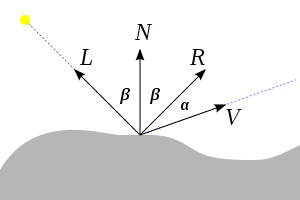
\includegraphics[width=0.8\textwidth]{images/phong-shading-model.png}
    \caption{Phong-Model-Specular}\label{Phong-Model-Specular}
\end{figure}

图\ref{Phong-Model-Specular}中的$\alpha$ 很小时,就是高光效果

\begin{align*}
    R = -L + 2(L \cdot N) * N \\
    I_{spec}=Ks * Il * (dot(V, R))^N_{s}
\end{align*}

Ks为镜面反射系数,Ns为高光指数。

\begin{figure}[htbp]
    \centering
    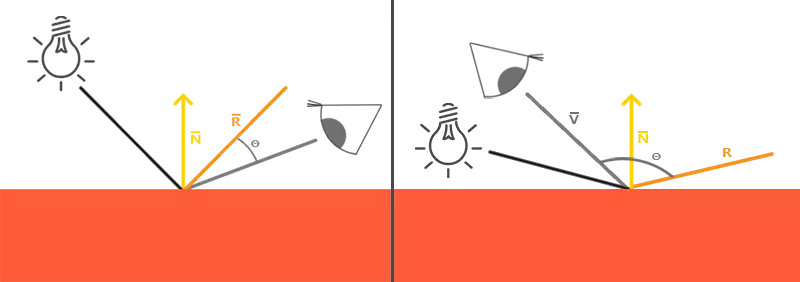
\includegraphics[width=0.8\textwidth]{images/classical-phong.png}
    \caption{Phong-Problem}\label{Phong-Problem}
\end{figure}
图\ref{Phong-Problem}模型中存在一个问题就是$\alpha$的角度大于90度时,会导致结果为负,产生假象。

Blinn-Phong是基于Phong的修正模型,

\begin{figure}[htbp]
    \centering
    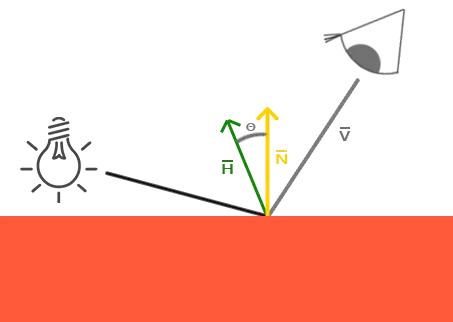
\includegraphics[width=0.8\textwidth]{images/blinn-phong.png}
    \caption{Blinn-Phong}\label{Blinn-Phong}
\end{figure}

图\ref{Blinn-Phong}通过半角来方法来解决可能出现角度大于90度的问题。

\begin{align*}
    H = \frac{L + V}{|L + V|}, \\
    I_{spec} = Ks * Il * (dot(N, H))^N_{s}
\end{align*}

H是入射光线方向L与视线方向V的中间向量,称之为半角向量。Classical-Phong更真实,Blinn-Phong高光更柔和,且计算速度较快,
实际中应用更广,OpenGL和DirectX渲染管线中是默认渲染模型。

\section{Global Illumination}
现实中的物体表面会接收大部分或全部来自其他反射出来的光线,称为indirect lighting或mutual illumination。
局部光照模型只考虑光对物体的照明,忽略了物体间的相互影响,其一般公式可以表示为

\begin{align*}
    I = I_{abmient} + \sum_{i}^{N}I_{light}\frac{1}{k_{c}+k_{l} \cdot d_{i} + k_{q} \cdot d_{i}^2}
    \left[ k_{d}(N \cdot L) + k_{s}(R \cdot V)^n \right]
\end{align*}

每个光源对物体的影响主要包括漫反射和镜面反射两部分,局部照明的阴影算法需要单独考虑。
\newline
全局照明考虑更全面,它自带阴影效果。它主要有两种算法:
\begin{itemize}
    \item {光线追踪法, 关注于镜面反射光,可严格追踪反射光线的方向,实际中采用逆向追踪法,减少计算量}
    \item {辐射度法, 关注于漫反射光,}
\end{itemize}
基本模型是 
\newline

\begin{align*}
    I_r = I_{ia}R_{a} + \sum_{l}I_{il}(N \cdot L_{l})d \omega_{il}(sR_{s} + dR_{d})
\end{align*}

其中的环境光和漫反射分量不依赖于观察者的位置View's Position。假设表面是由微面元组成microfacet,其镜面分量为:
\newline

\begin{align*}
    R_s = \frac{F}{\pi} \frac{DG}{\pi (N \cdot L)(N \cdot V)}
\end{align*}

为更加丰富,引入了几何项G,Fresnel项F,粗糙度项D。
\newline

\textbf{粗糙度项D},代表了可以有效反射光的那一部分微面元所占的比例,有多种分别函数。
高斯分布模型
\newline

\begin{align*}
    D = ce^{-(\alpha / m)^2}
\end{align*}

Bechmann分布函数
\newline

\begin{align*}
    D = \frac{1}{m^2cos^4(\theta)}e^-(tan\alpha / m)^2
\end{align*}

\textbf{几何项G},几何衰减项,表现了微小面元之间的互相遮挡shadowing and masking所造成的影响。
\newline

\begin{align*}
    G = \left\{
        1, \frac{2(N \cdot H)(N \cdot V)}{(V \cdot H)}, \frac{2(N \cdot H)(N \cdot L)}{(V \cdot H)} 
    \right\}
\end{align*}

\textbf{Fresnel项F},描述了在每一个微面元上光是如何反射,与入射角和波长相关。
\newline

\begin{align*}
    c = cos(\theta) = V \cdot H \\
    g^2 = n^2 + c^2 - 1 \\
F = \frac{1(g-c)^2}{2(g+c)^2} \left\{ 1+\frac{[c(g+c)-1]^2}{[c(g-c)+1]^2} \right\}
\end{align*}

\section{Physically based Rendering}

PBR refers to the concept of using realistic shading/lighting models along with measured surface values to accurately represent real-world materials

\section{notes}

多边形渲染会降低渲染速度,而要丰富的表面就需要更多的细节,要模拟表面的凹凸感,
与其增加多边形,不如利用光照的明暗来表示凹凸感,骗过人眼。光照模型都跟光线向量和表面法向量的夹角有关。
扰动就是影响法线向量与光线向量的夹角发生变化,从而产生明暗的变化,给人凹凸感。这就是使用法线贴图在低模中获得高模的凹凸的表面光照效果
